\section{Approach}

In the next section we describe our solution for the distributed lighting problem. The main components of our system are the Local Controller, used to maintain the illuminance at each desk at the desired reference, the Simplex Algorithm, that calculates the optimal solution to the linear programm that describes this problem, and the TCP/IP Server, which serves as an intermediary between the clients and the system. An overview of the system is depicted on Figure \ref{fig:global_system}.

\begin{figure}[!ht]
    \centering
        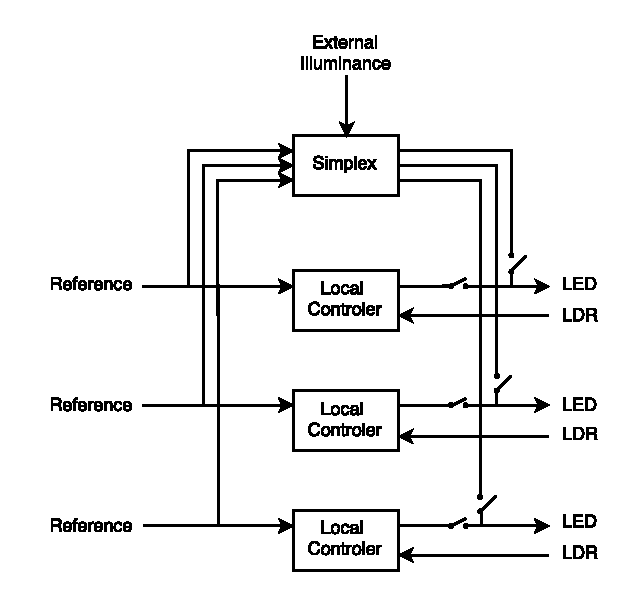
\includegraphics[scale=0.8]{img/GlobalSystem}
    \caption{Block diagram of the implemented system}\label{fig:global_system}
\end{figure}

\subsection{Physical Setup}
\label{sec:PhysicalSetup}


The setup must model a room with luminaires on its ceiling. Each luminaire has a controller that keeps the light below it above some standard level of illuminance. For this project it was pre-established that the room contained three luminaires.

For the physical setup a wooden box was used. This was preferred to a cardboard box because of the increased sturdiness. Since the controllers (Arduinos) are too big to be included inside the luminaires in our model they were put on the outside of the box,  and all the wiring is done outside the box using a breadboard (see \autoref{fig:setup_box_closed}). Both the breadboard and the Arduinos are screwed to the box preventing them to move, which could easily disconnect the jumpers. Tight holes were made to pass the wires needed to light the LED and read the sensor, while preventing light from entering the box (see \autoref{fig:setup_arduino_connections}).

\begin{figure}[h]
    \centering
    \begin{subfigure}[t]{0.49\textwidth}
        \centering
        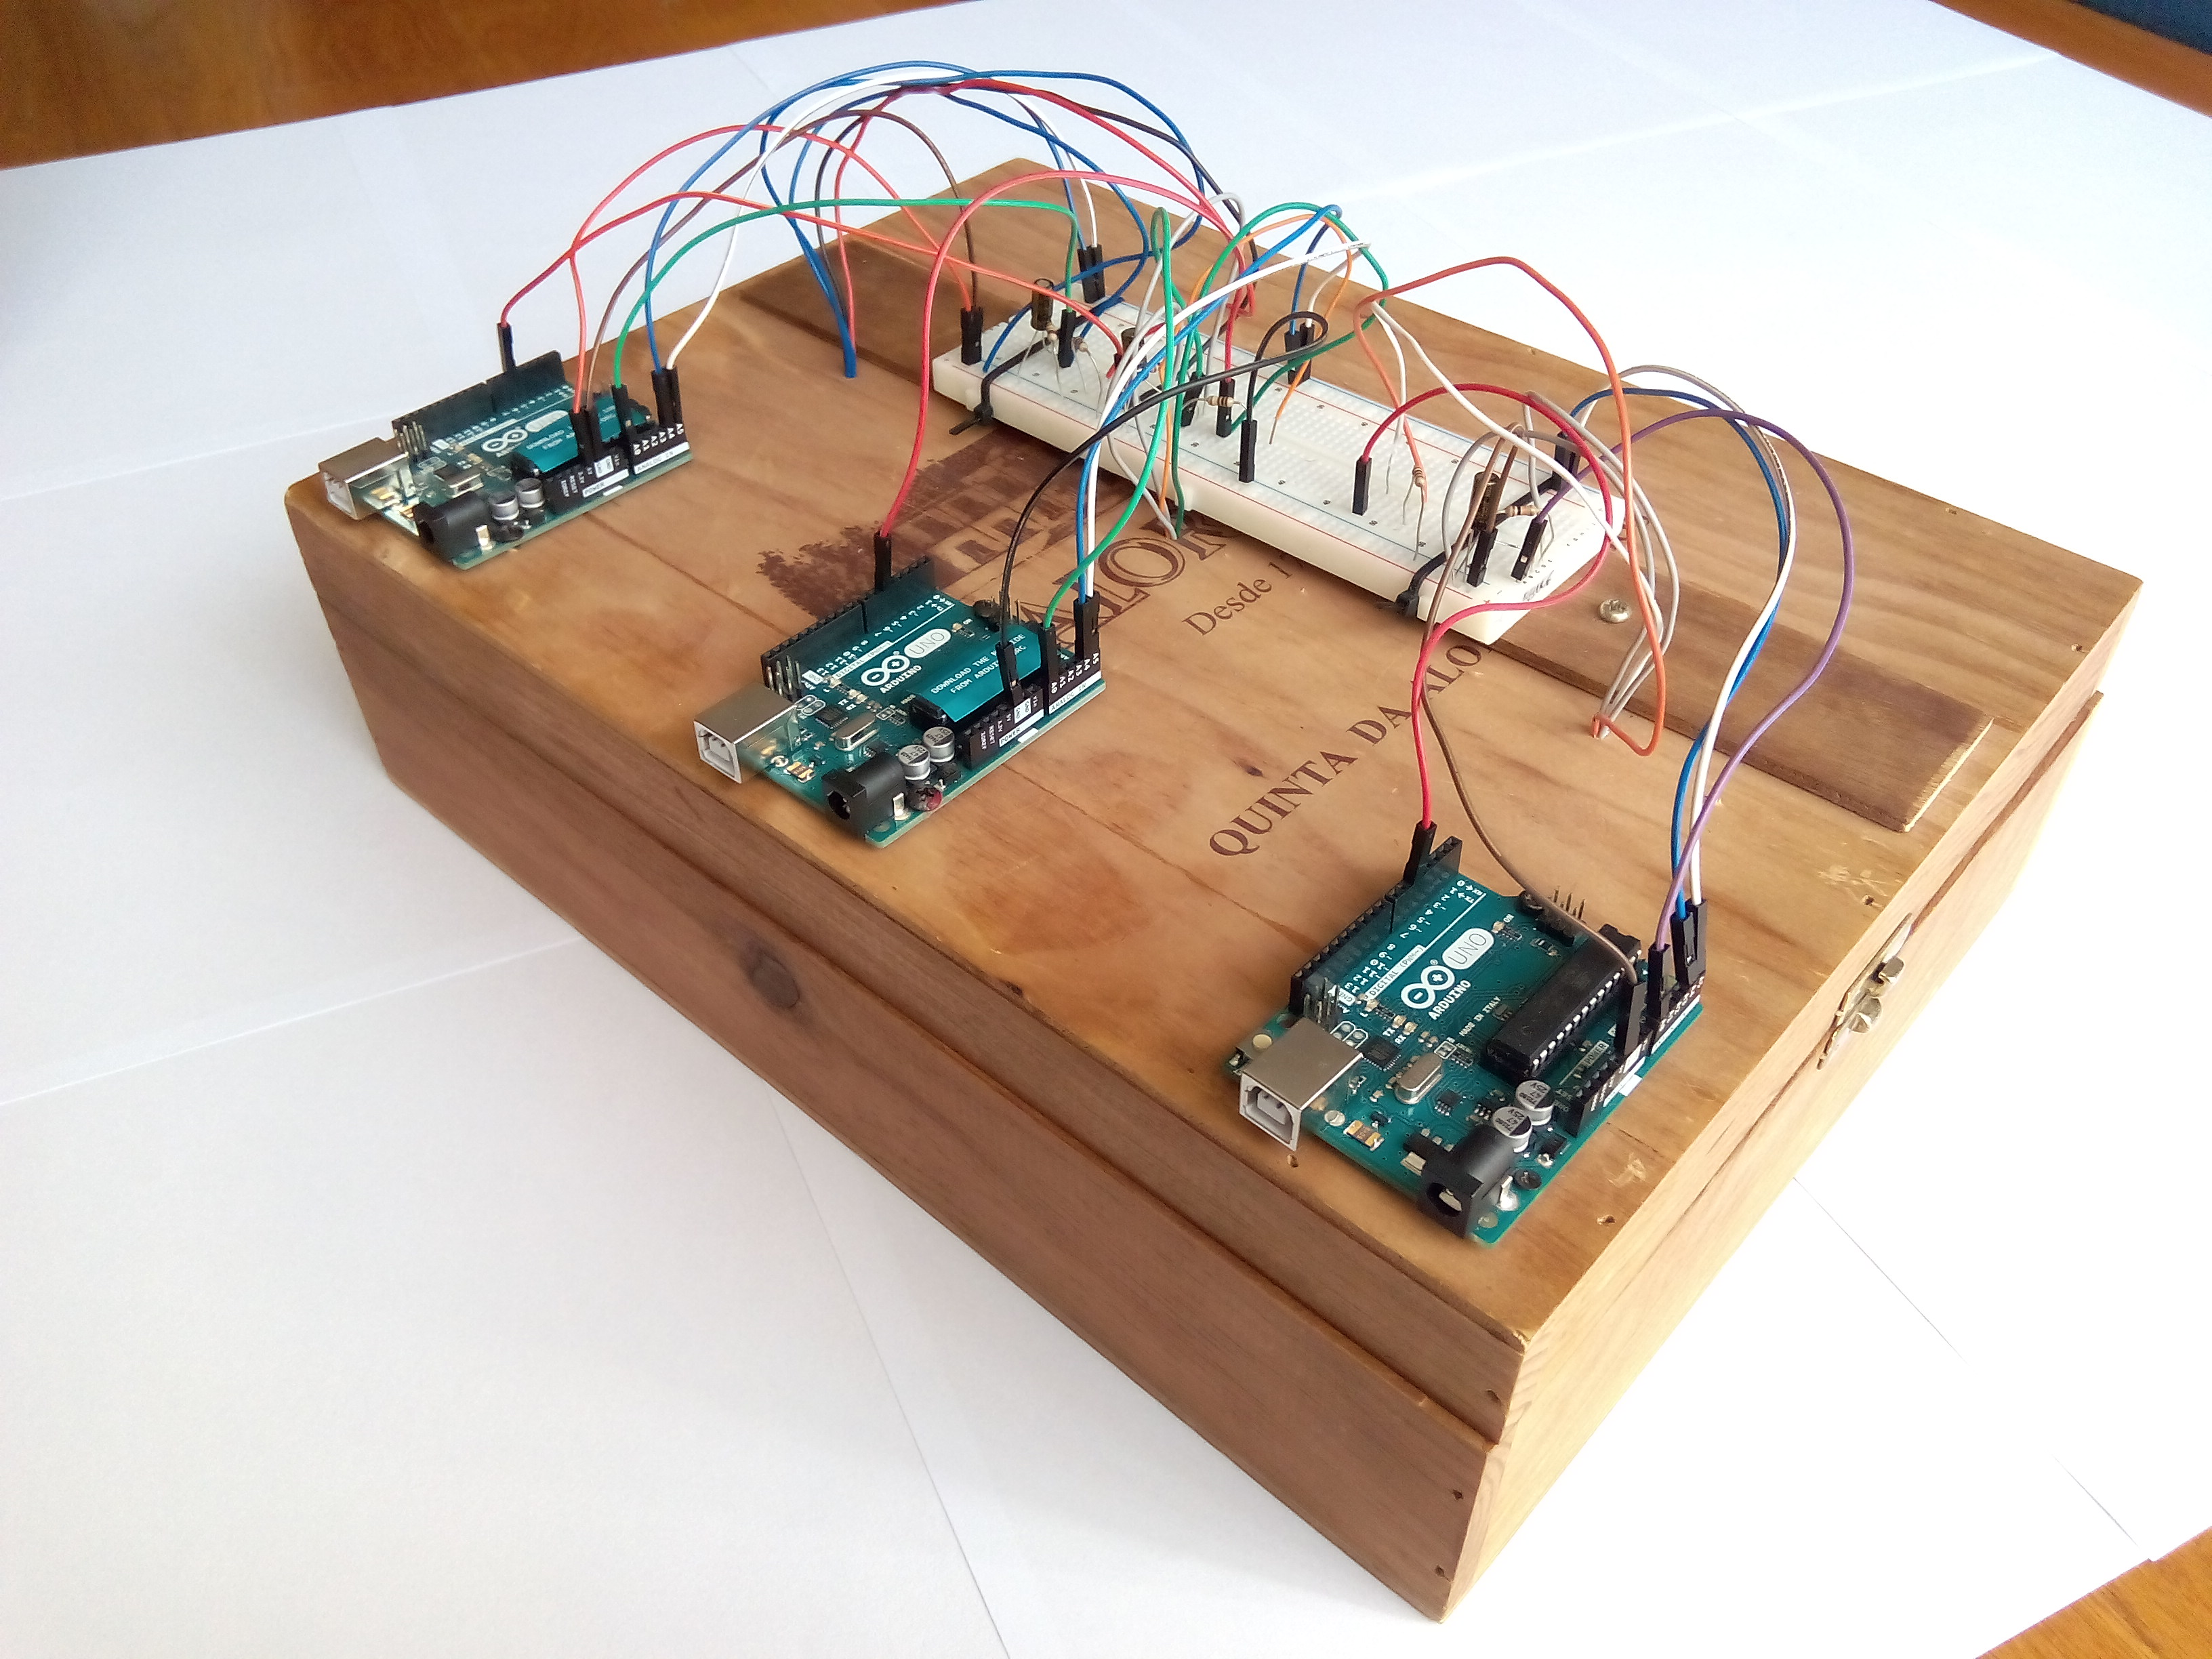
\includegraphics[width=\textwidth]{img/setup_box_closed}
        \caption{Arduinos and breadboard on top of the box}
        \label{fig:setup_box_closed}
    \end{subfigure}
    \begin{subfigure}[t]{0.49\textwidth}
        \centering
        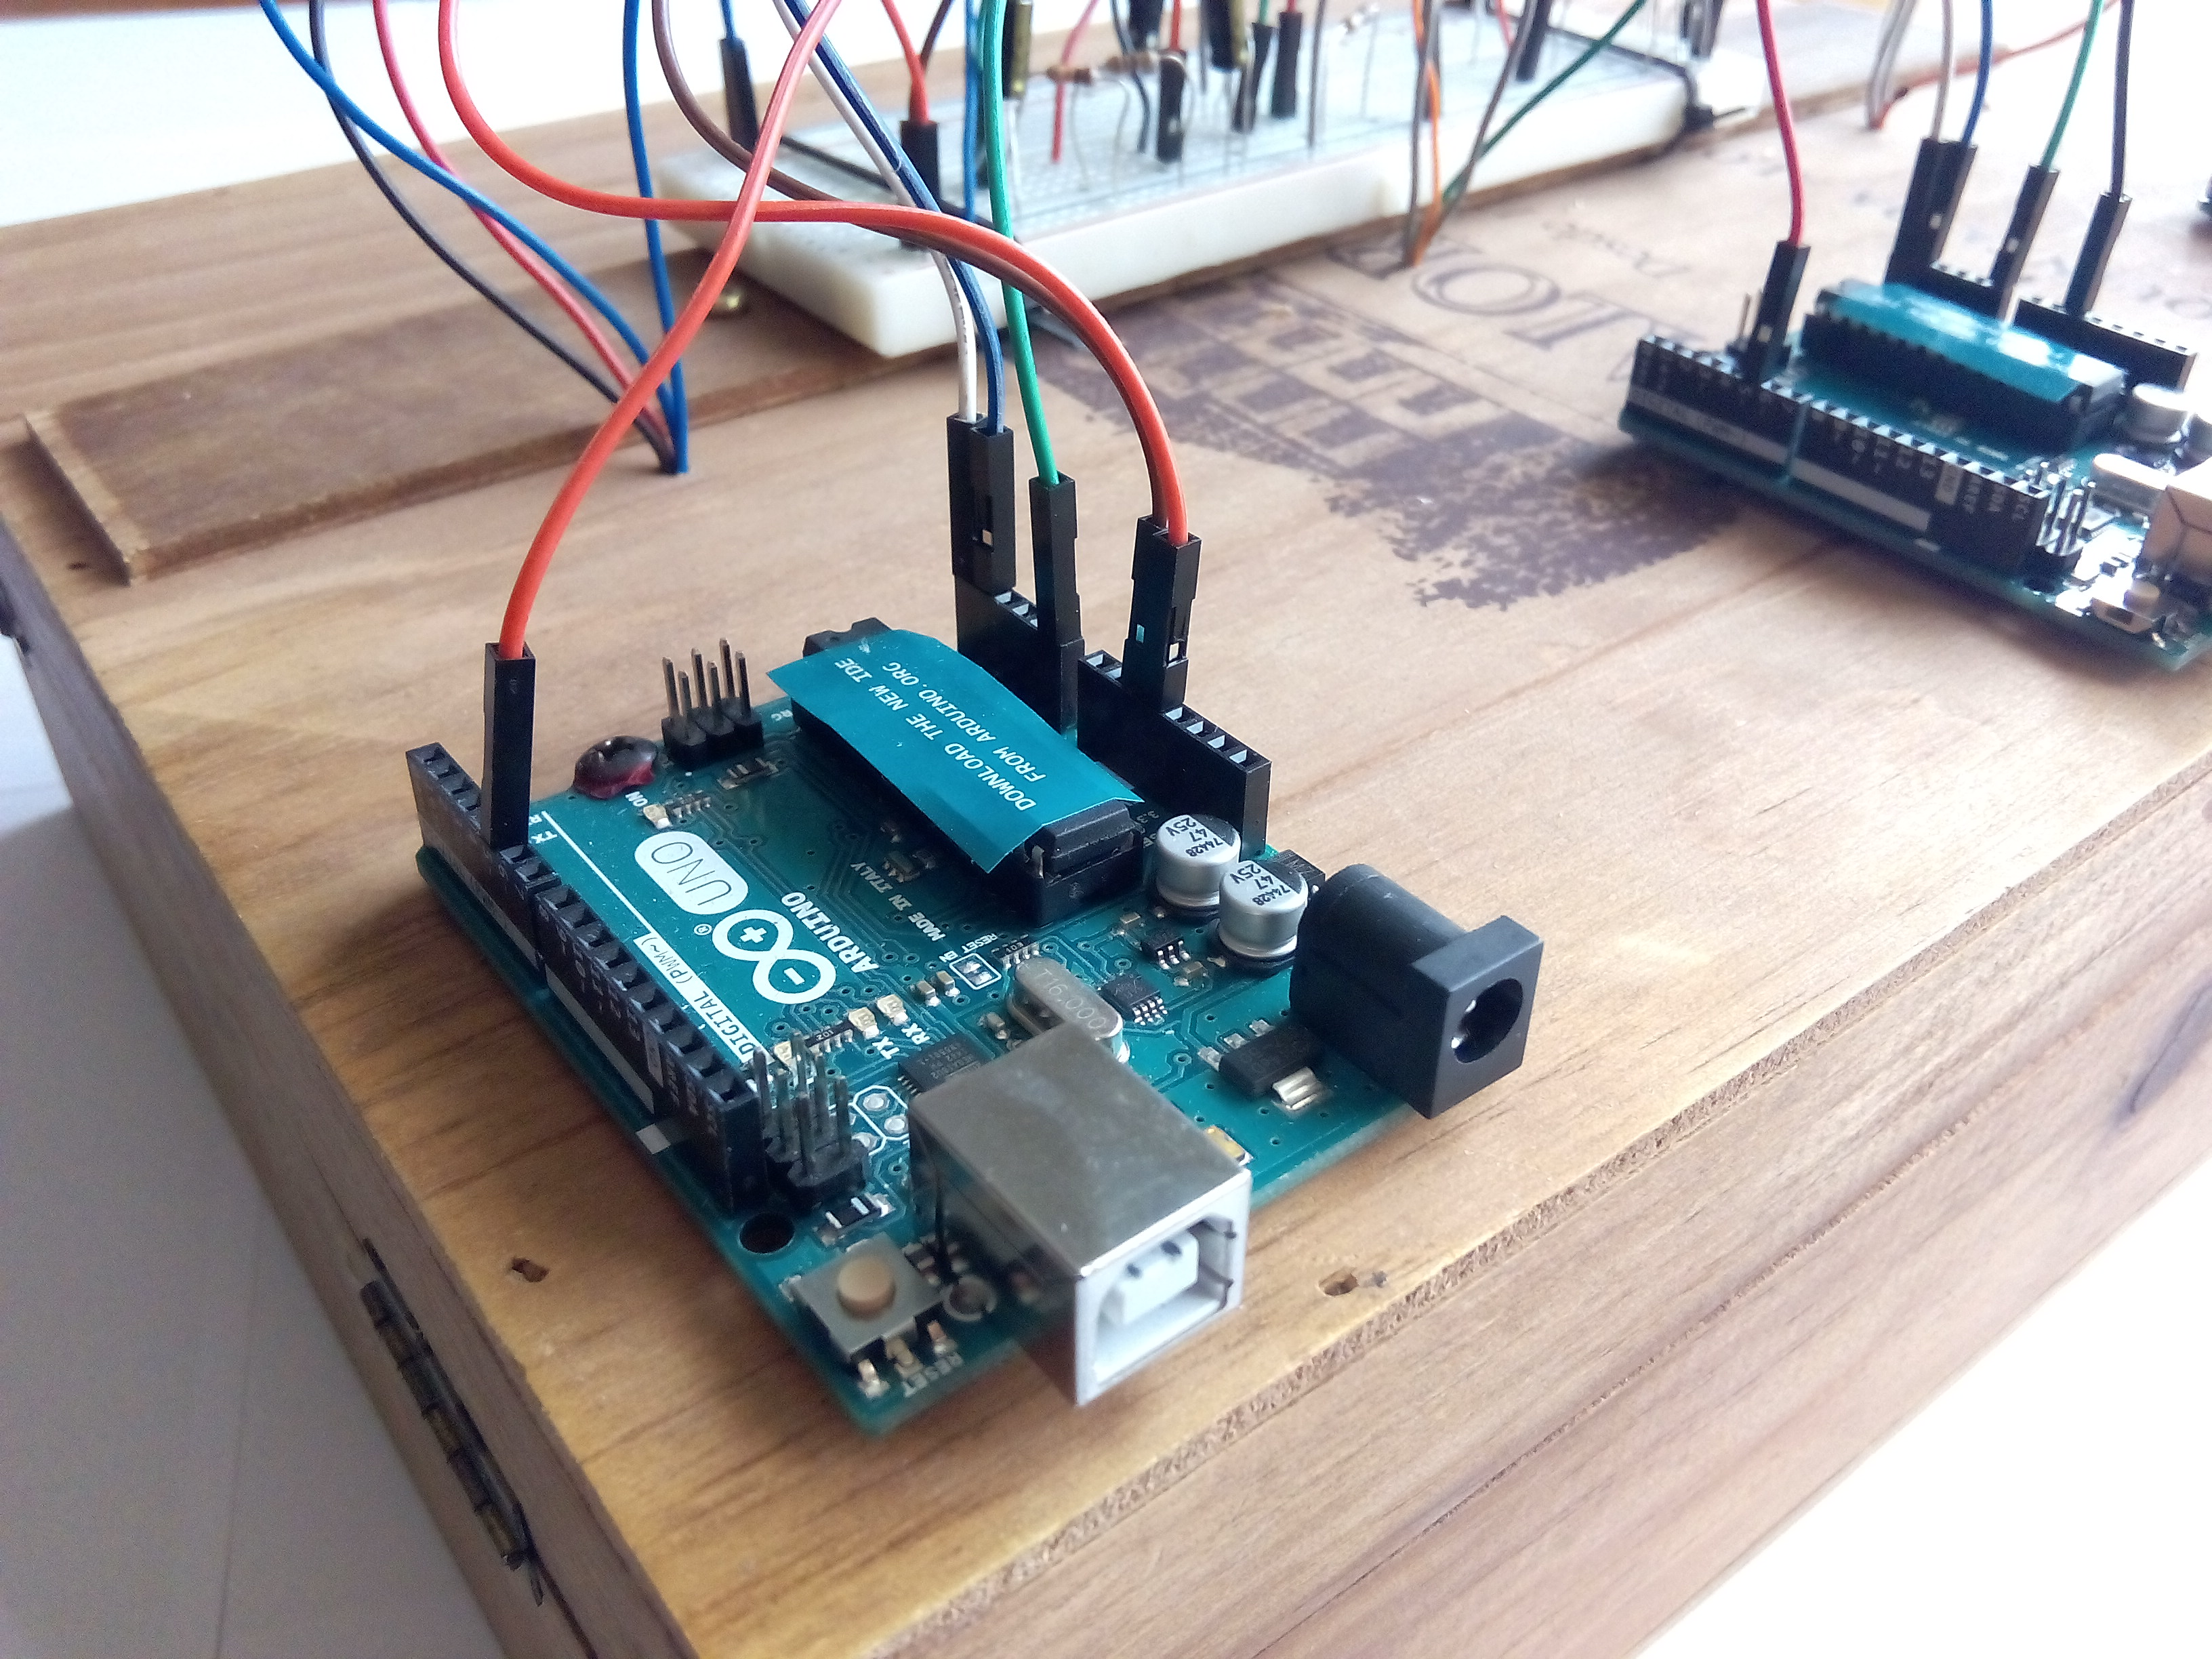
\includegraphics[width=\textwidth]{img/setup_arduino_connections.jpg}
        \caption{Detail showing the connections on the Arduino and one hole in the box}
        \label{fig:setup_arduino_connections}
    \end{subfigure}
    \caption{The outside of the box}
    \label{fig:setup_box_outside}
\end{figure}


On the inside of the box only the luminaires are present. Each luminaire is assumed to include both a LED light and a light sensor (LDR). The LED and the LDR are separated by a piece of cardboard so that the light from the LED does not directly affect the LDR reading (\autoref{fig:setup_box_open}). Only reflected light should be read. In order to increase the light reflection inside the box --- so that the LDR senses more light --- a white sheet of paper was placed on the bottom of the box (see \autoref{fig:setup_LDR_LED}).

\begin{figure}[h]
    \centering
    \begin{subfigure}[t]{0.49\textwidth}
        \centering
        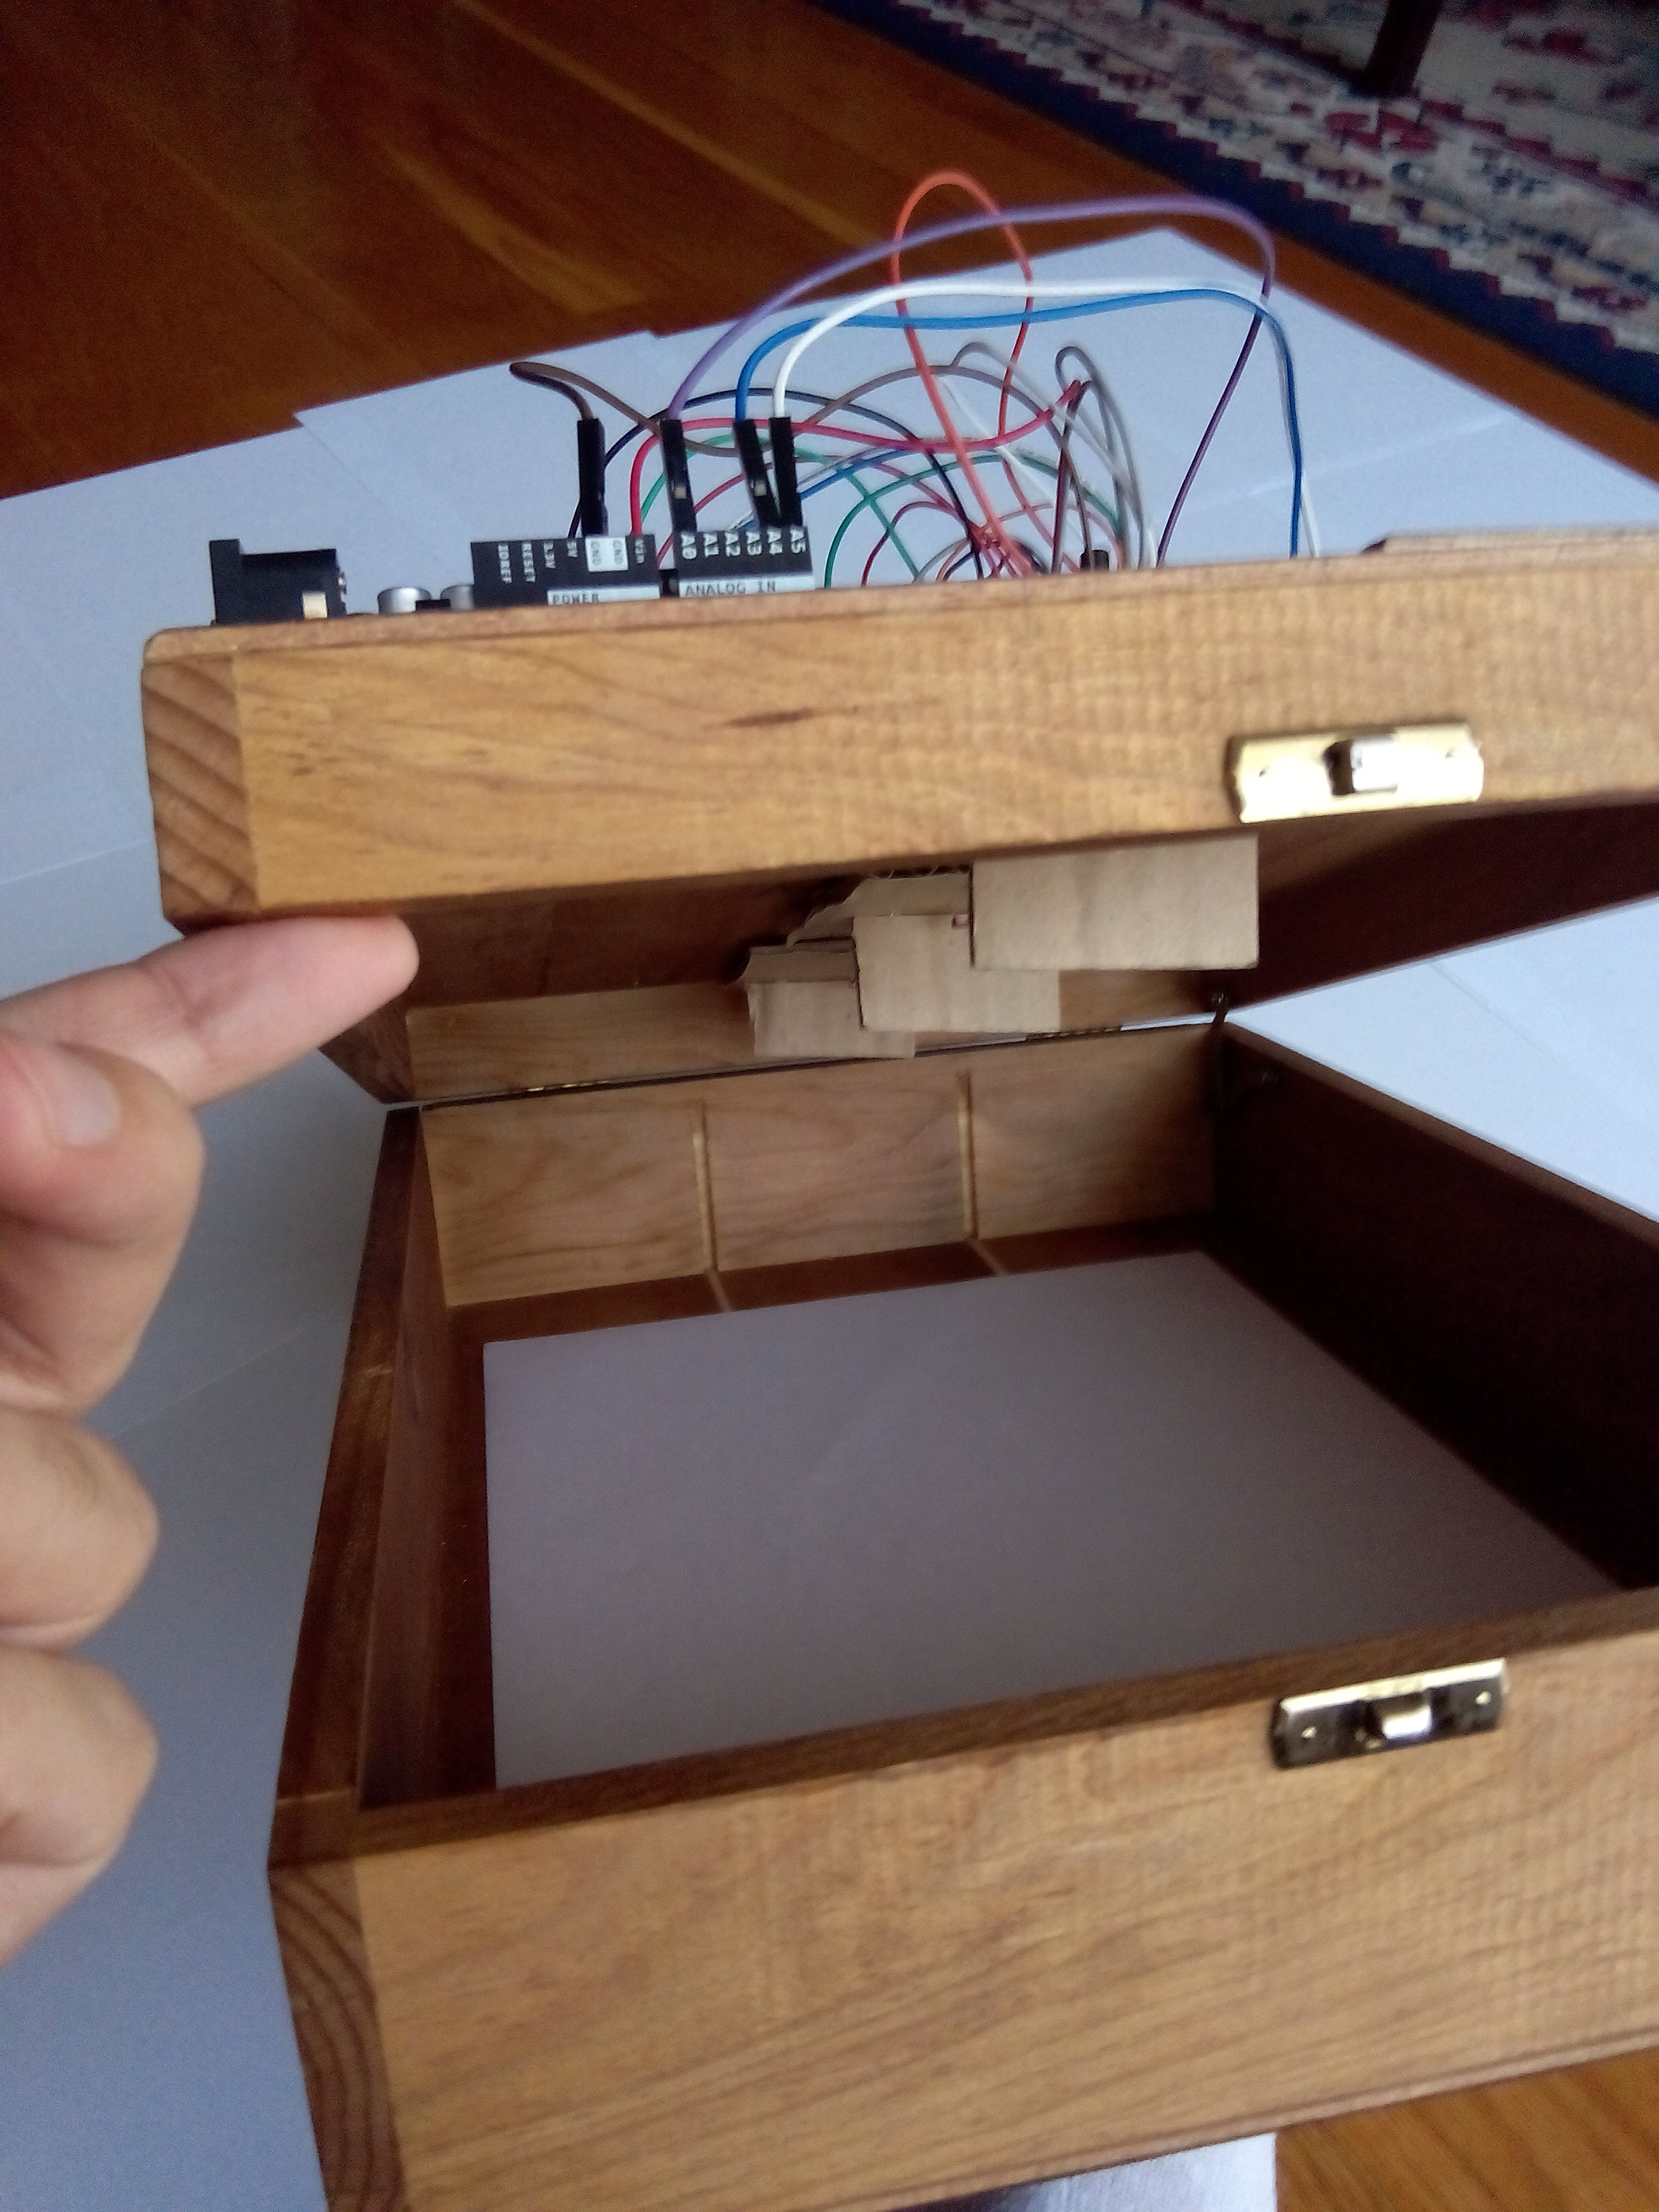
\includegraphics[width=\textwidth]{img/setup_box_open}
        \caption{Luminaires on the ceiling and white sheet on the floor}
        \label{fig:setup_box_open}
    \end{subfigure}
    \begin{subfigure}[t]{0.49\textwidth}
        \centering
        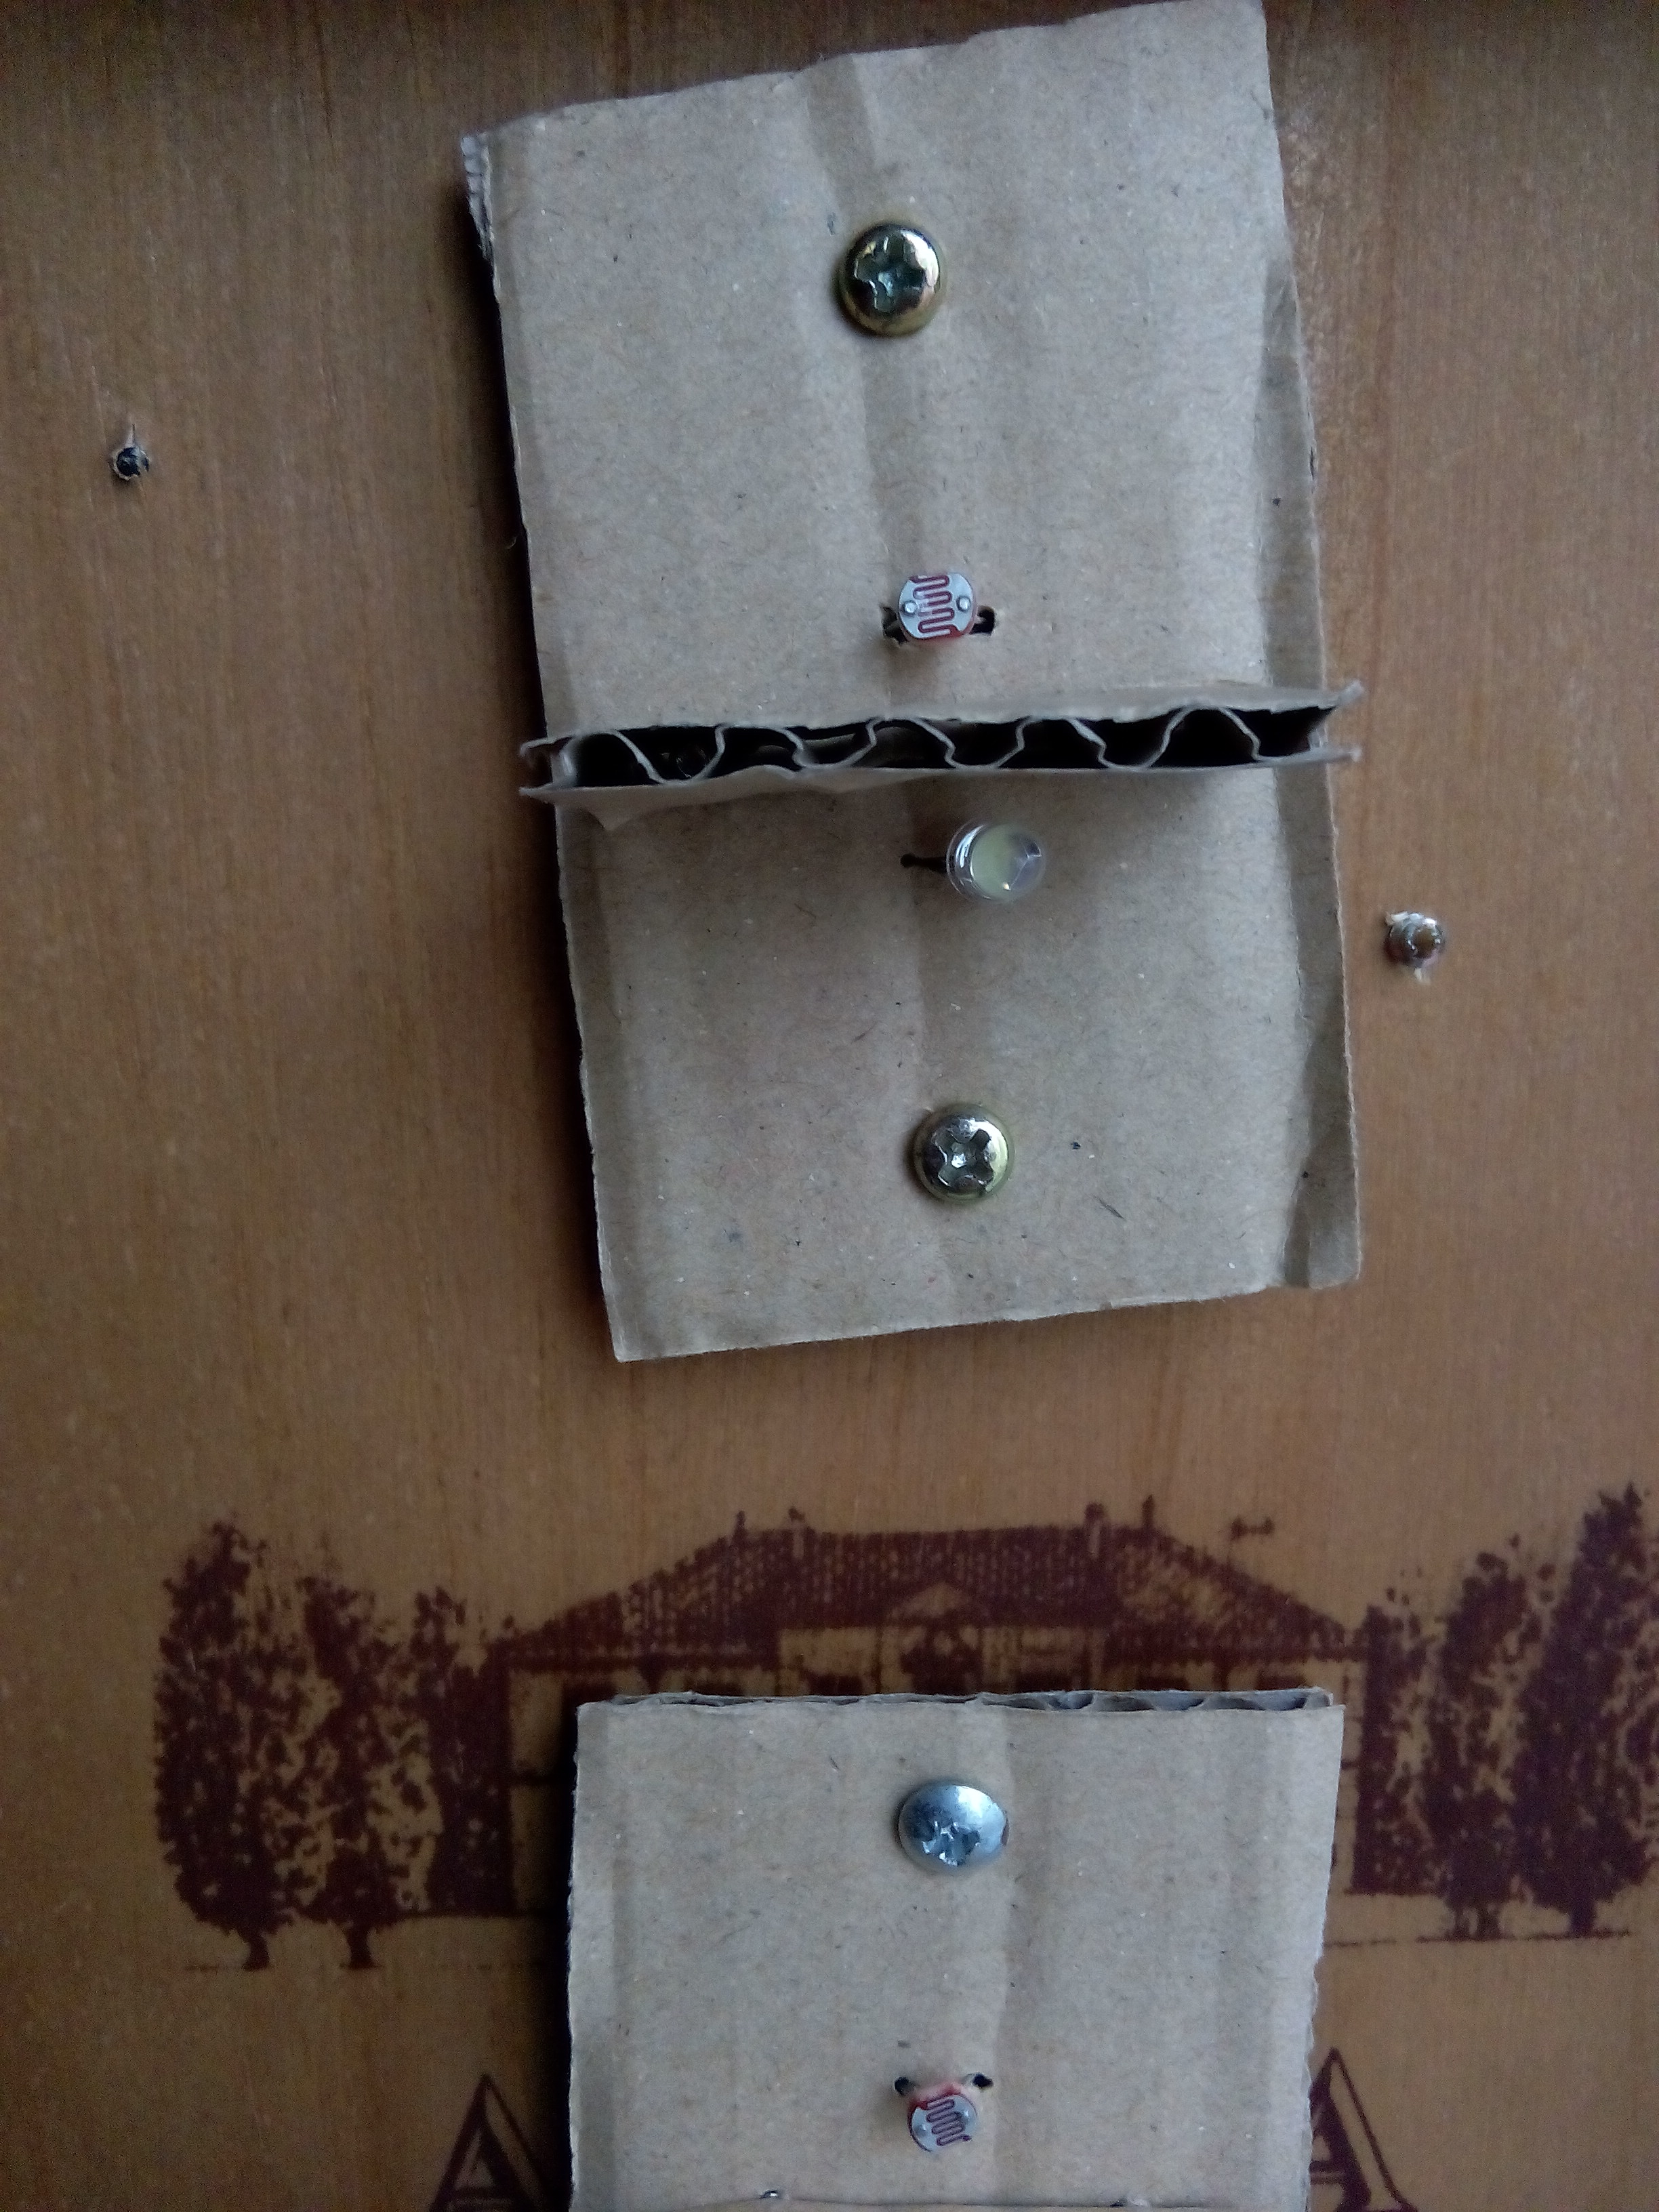
\includegraphics[width=\textwidth]{img/setup_LDR_LED}
        \caption{Detail of a luminaire. The LDR on top, LED on bottom and cardboard in between}
        \label{fig:setup_LDR_LED}
    \end{subfigure}
    \caption{The inside of the box}
    \label{fig:setup_box_inside}
\end{figure}

The assignment requires that the model has a window. The used box has hinges and the top of the box can be opened (see \autoref{fig:setup_LDR_LED}). Therefore this was used as an window. The top should only be opened in small angles so that we can consider (by approximation) that the LDR is still facing the ground and that the light of the LED is mostly reflected back at the LDR.

% about the circuits

The emitter-detector circuit for each luminaire is shown in \autoref{fig:setup_circuits}. The emitter is made of an LED in series with a current limiting resistor (\autoref{fig:setup_LED_circuit}). The typical forward voltage of the used LED is \SI{3.0}{\volt} and its maximum forward current is \SI{20}{\milli\ampere}. Since the Arduino is powered with \SI{5}{\volt} the voltage on pin \texttt{D5} is at most \SI{5}{\volt}. Therefore, using a \SI{100}{\ohm} resistor makes the LED be at its maximum power when the duty cycle on pin \texttt{D5} is 1. For the light detector circuit a voltage divider is used, consisting of a normal resistor and a photoresistor. A capacitor is also included in parallel with the resistor to act as a low-pass filter to eliminate noise from the readings. An analysis of the characteristic of the LDR is made in \ref{subsubsec:LDR_model}.

\begin{figure}[h]
    \centering
    \begin{subfigure}[t]{0.49\textwidth}
        \centering
        \begin{circuitikz} \draw
            (0,0) node[sground] {}
            to[resistor, l_=\mbox{$R_1 = \SI{100}{\ohm}$}] (0,2);
            \draw (0,4) to[empty led, l=$D_1$] (0,2) ;
			\draw (0,4) to[short, -o] (-1.5,4)
            node[left]{\texttt{D5}}
            ;
        \end{circuitikz}
        \caption{The LED circuit. Pin \texttt{D5} controls the power on the LED using PWM.}
        \label{fig:setup_LED_circuit}
    \end{subfigure}
    \begin{subfigure}[t]{0.49\textwidth}
        \centering
        \begin{circuitikz} \draw
            (0,0) node[sground] {}
            to[resistor, l=\mbox{$R_3 = \SI{10}{\kilo\ohm}$}] (0,2)
            to[photoresistor, l=$R_2$] (0,4)
            to[short, -o] (0,4.5)
            node[right]{$V_S = 5 V$}

            (1,0) node[sground] {}
            to[polar capacitor, l_=\mbox{$C_1 = \SI{1}{\micro\farad}$}] (1,2)
            (0,2) -- (1,2)

            (1,2) to[short, -o] ++(2,0)
            node[right]{\texttt{A0}}
            ;
        \end{circuitikz}
        \caption{The light detector. An LDR is used and readings are done on pin \texttt{A0}.}
        \label{fig:setup_LDR_circuit}
    \end{subfigure}
    \caption{Emitter-detector circuitry of each luminaire}
    \label{fig:setup_circuits}
\end{figure}

A I\textsuperscript{2}C/TWI bus is used to implement the communications between the controllers of each luminaire. The physical implementation of this bus is attained by connecting the \texttt{A4} pin of all the Arduinos as well as the \texttt{A5} pins --- SDA and SCL respectively.

\subsection{System Characteristics}
\label{sec:SystemCharacteristics}

\subsubsection{Steady State}
\label{sub:SteadyState}

The steady state response of the system was determined by setting the duty cycle of the LED to all values in the PWM range 0--255. \textcolor{red}{Each sample was acquired \SI{200}{\milli\second} after the previous one so that the system had time to reach a steady state. This is an adequate time between samples because $RC$ constant of the detector circuit in \autoref{fig:setup_LDR_circuit} is $\tau = R_2C_1 = \SI{60}{\milli\second}$ and \SI{400}{\milli\second} amounts to more than $3\tau$. The reason why $R_2$ is in the time constant and not $R_3$ is because the PWM value was incremented and hence $C_1$ charges via $R_2$. If the data was acquired while decrementing the PWM value $R_3$ would be used instead.}

% explain R_2's value above?

A graph of the acquired data can be seen in \autoref{fig:steady_state}. We conclude that the resistance of the LDR does not vary linearly with the duty cycle on the LED. Nonetheless it is possible to obtain a linear function relating the input an output of the system, as described in \ref{subsubsec:LDR_model}.

\begin{figure}[h]
    \centering
    \resizebox{\textwidth}{!}{% Title: glps_renderer figure
% Creator: GL2PS 1.3.8, (C) 1999-2012 C. Geuzaine
% For: Octave
% CreationDate: Tue Dec 29 23:09:54 2015
\setlength{\unitlength}{1pt}
\begin{picture}(0,0)
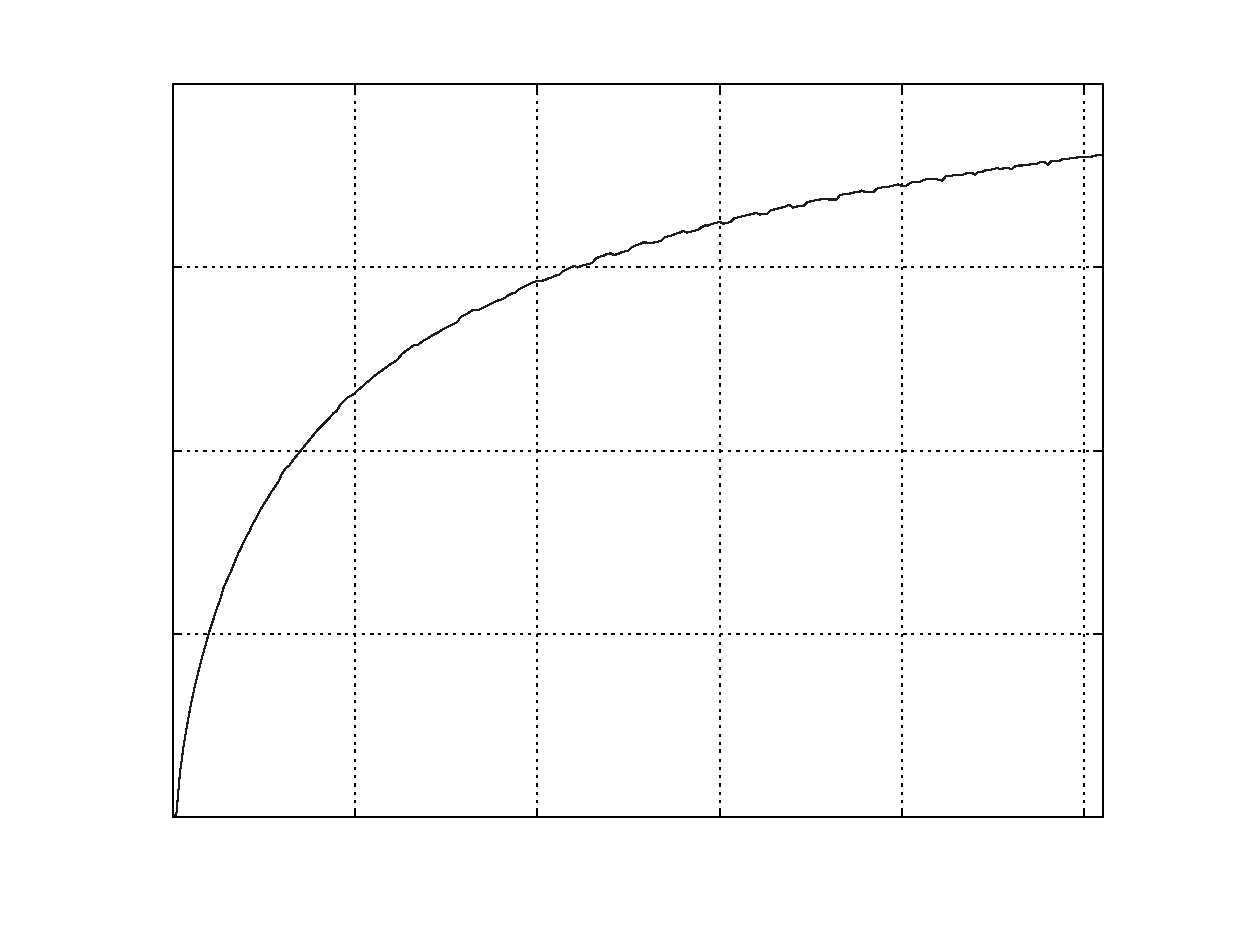
\includegraphics{img/steady_state-inc}
\end{picture}%
\begin{picture}(576,432)(0,0)
\fontsize{10}{0}
\selectfont\put(74.88,42.5189){\makebox(0,0)[t]{\textcolor[rgb]{0,0,0}{{0}}}}
\fontsize{10}{0}
\selectfont\put(162.409,42.5189){\makebox(0,0)[t]{\textcolor[rgb]{0,0,0}{{50}}}}
\fontsize{10}{0}
\selectfont\put(249.939,42.5189){\makebox(0,0)[t]{\textcolor[rgb]{0,0,0}{{100}}}}
\fontsize{10}{0}
\selectfont\put(337.468,42.5189){\makebox(0,0)[t]{\textcolor[rgb]{0,0,0}{{150}}}}
\fontsize{10}{0}
\selectfont\put(424.998,42.5189){\makebox(0,0)[t]{\textcolor[rgb]{0,0,0}{{200}}}}
\fontsize{10}{0}
\selectfont\put(512.527,42.5189){\makebox(0,0)[t]{\textcolor[rgb]{0,0,0}{{250}}}}
\fontsize{10}{0}
\selectfont\put(69.8755,47.52){\makebox(0,0)[r]{\textcolor[rgb]{0,0,0}{{0}}}}
\fontsize{10}{0}
\selectfont\put(69.8755,135.54){\makebox(0,0)[r]{\textcolor[rgb]{0,0,0}{{1}}}}
\fontsize{10}{0}
\selectfont\put(69.8755,223.56){\makebox(0,0)[r]{\textcolor[rgb]{0,0,0}{{2}}}}
\fontsize{10}{0}
\selectfont\put(69.8755,311.58){\makebox(0,0)[r]{\textcolor[rgb]{0,0,0}{{3}}}}
\fontsize{10}{0}
\selectfont\put(69.8755,399.6){\makebox(0,0)[r]{\textcolor[rgb]{0,0,0}{{4}}}}
\fontsize{10}{0}
\selectfont\put(298.08,31.5188){\makebox(0,0)[t]{\textcolor[rgb]{0,0,0}{{PWM value (0--255)}}}}
\fontsize{10}{0}
\selectfont\put(59.8755,223.56){\rotatebox{90}{\makebox(0,0)[b]{\textcolor[rgb]{0,0,0}{{Voltage at \texttt{A0} (\si{\volt})}}}}}
\end{picture}
}
    \caption{Steady state voltage at pin \texttt{A0} as a function of the duty cycle of the LED}
    \label{fig:steady_state}
\end{figure}

\subsubsection{Modeling the LDR}
\label{subsubsec:LDR_model}

Since the steady state plot in \autoref{fig:steady_state} reveals that the system is nonlinear it is useful to understand why. The main sources from nonlinearity should result from the LED, the LDR or a combination of both.

% TODO put full datasheet in an annex?

With that in mind the LDR datasheet was analysed. On it the graph in \autoref{fig:LDR_datasheet} can be found. This graph gives a range of values for the resistance of the LDR for each value of incident illuminance. To produce an equation that models the LDR resistance as a function of illuminance the resistance value used for the model is the mean of the maximum and minimum values given for each illuminance. The final result should be a function which produces a line that crosses the middle of the dark region in \autoref{fig:LDR_datasheet}. Note the axis of the figure are both in logarithmic scale. The considered points to obtain this linear function (in a log-log reference) were $(L_1, R_1) = (\SI{100}{\lux}; \SI{2.5}{\kilo\ohm})$ and $(L_2, R_2) = (\SI{1}{\lux}; \SI{60}{\kilo\ohm})$. The model will be an equation in the form
\begin{equation} \label{eq:log-log_line}
    \log_{10} R_{LDR} = a \log_{10} L + b.
\end{equation}

\begin{figure}[h]
    \centering
    \begin{subfigure}[t]{0.39\textwidth}
	\centering
	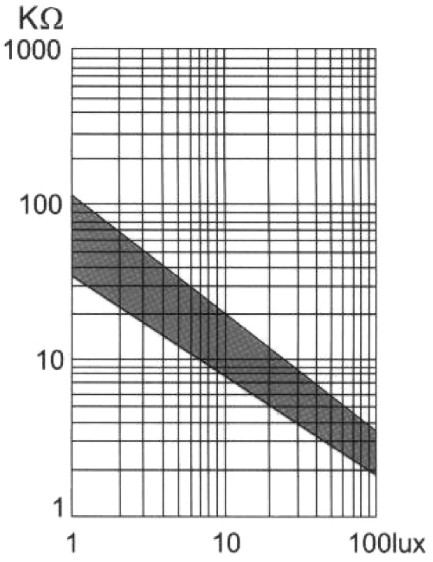
\includegraphics[width=.95\textwidth]{img/LDR_datasheet}
	\caption{LDR resistance as a function of illuminance according to the GL5528's datasheet}
	\label{fig:LDR_datasheet}
    \end{subfigure}
    \begin{subfigure}[t]{0.59\textwidth}
	\centering
	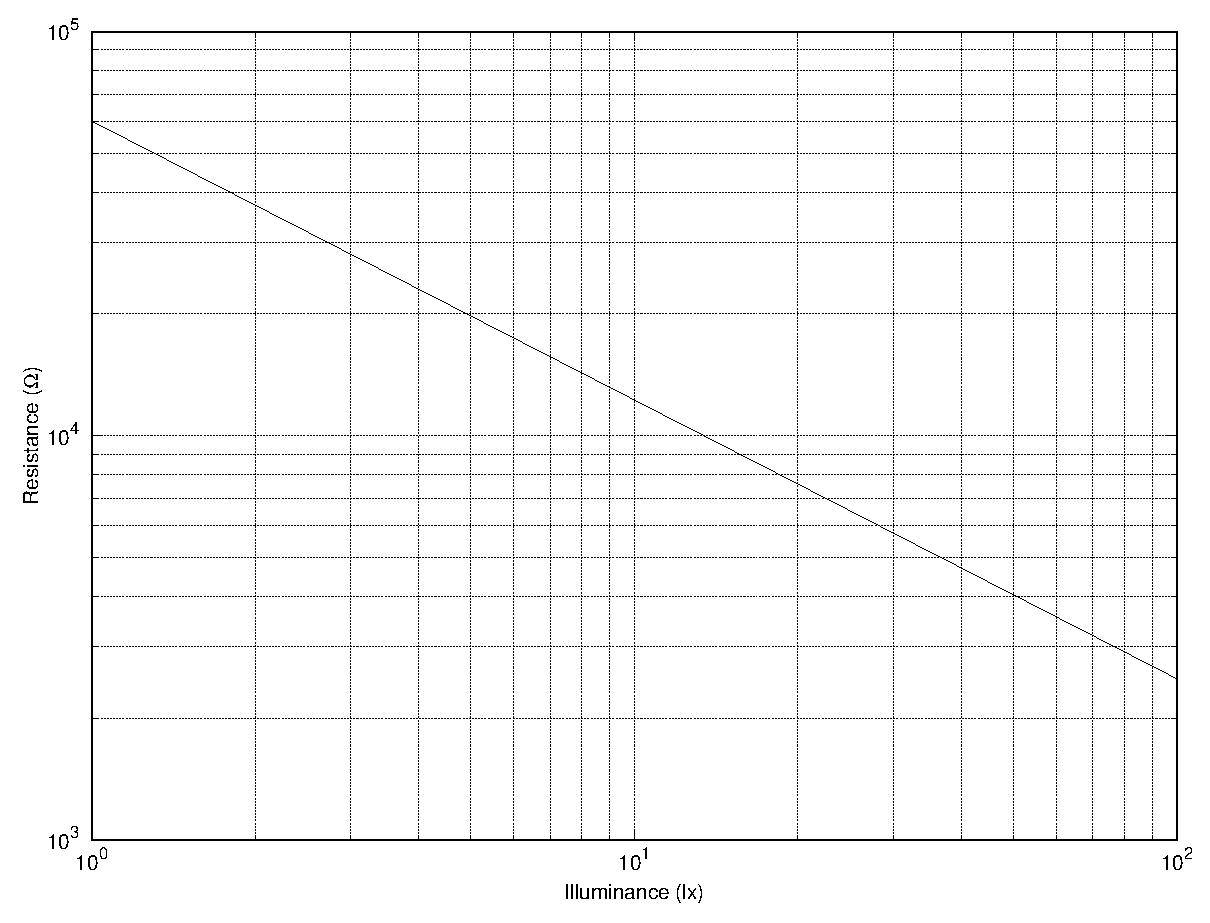
\includegraphics[width=.95\textwidth]{img/LDR_model}
	\caption{Model for the resistance of the LDR as function of the incident illuminance}
	\label{fig:LDR_model}
    \end{subfigure}
    \caption{LDR characteristic}
    %\label{fig:LDR_characteristic}
\end{figure}


We can substitute $(L_1, R_1)$ and $(L_2, R_2)$ in \eqref{eq:log-log_line} to obtain the system of equations
\begin{equation} \label{eq:log-log_line_system}
    \begin{bmatrix}
	\log_{10}R_1 \\ \log_{10}R_2
    \end{bmatrix}
    =
    \begin{bmatrix}
	\log_{10}L_1  &  1 \\
	\log_{10}L_2  &  1
    \end{bmatrix}
    \begin{bmatrix}
	a \\ b
    \end{bmatrix}.
\end{equation}
By solving the system the values $a \approx -0.6901$ and $b \approx 4.7782$ are obtained for this case.

With the values for $a$ and $b$ and \eqref{eq:log-log_line} it is possible to plot the graph in \autoref{fig:LDR_model} which models the LDR characteristic, as desired. Using \eqref{eq:log-log_line} it is possible to obtain the incident illuminance ($L$) from the resistance of the LDR $R_{LDR}$
\begin{equation} \label{eq:Rldr_to_lux}
    L = 10^{-\frac{b}{a}} R_{LDR}^{\frac{1}{a}} .
\end{equation}
And since in a steady state
\begin{equation} \label{eq:VA0_to_Rldr}
    R_{LDR} = \frac{V_S R_3}{V_{\texttt{A0}}} - R_3 ,
\end{equation}
we can substitute \eqref{eq:VA0_to_Rldr} in \eqref{eq:Rldr_to_lux} and apply the new equation to the plot in \autoref{fig:steady_state} to produce the plot in \autoref{fig:pwm_to_lux} which relates the duty cycle of the LED to the illuminance measured by the LDR. We can conclude that the illuminance varies linearly with the duty cycle applied to the LED.

\begin{figure}[h]
    \centering
    \resizebox{0.75\textwidth}{!}{% Title: glps_renderer figure
% Creator: GL2PS 1.3.8, (C) 1999-2012 C. Geuzaine
% For: Octave
% CreationDate: Mon Dec 28 19:17:53 2015
\setlength{\unitlength}{1pt}
\begin{picture}(0,0)
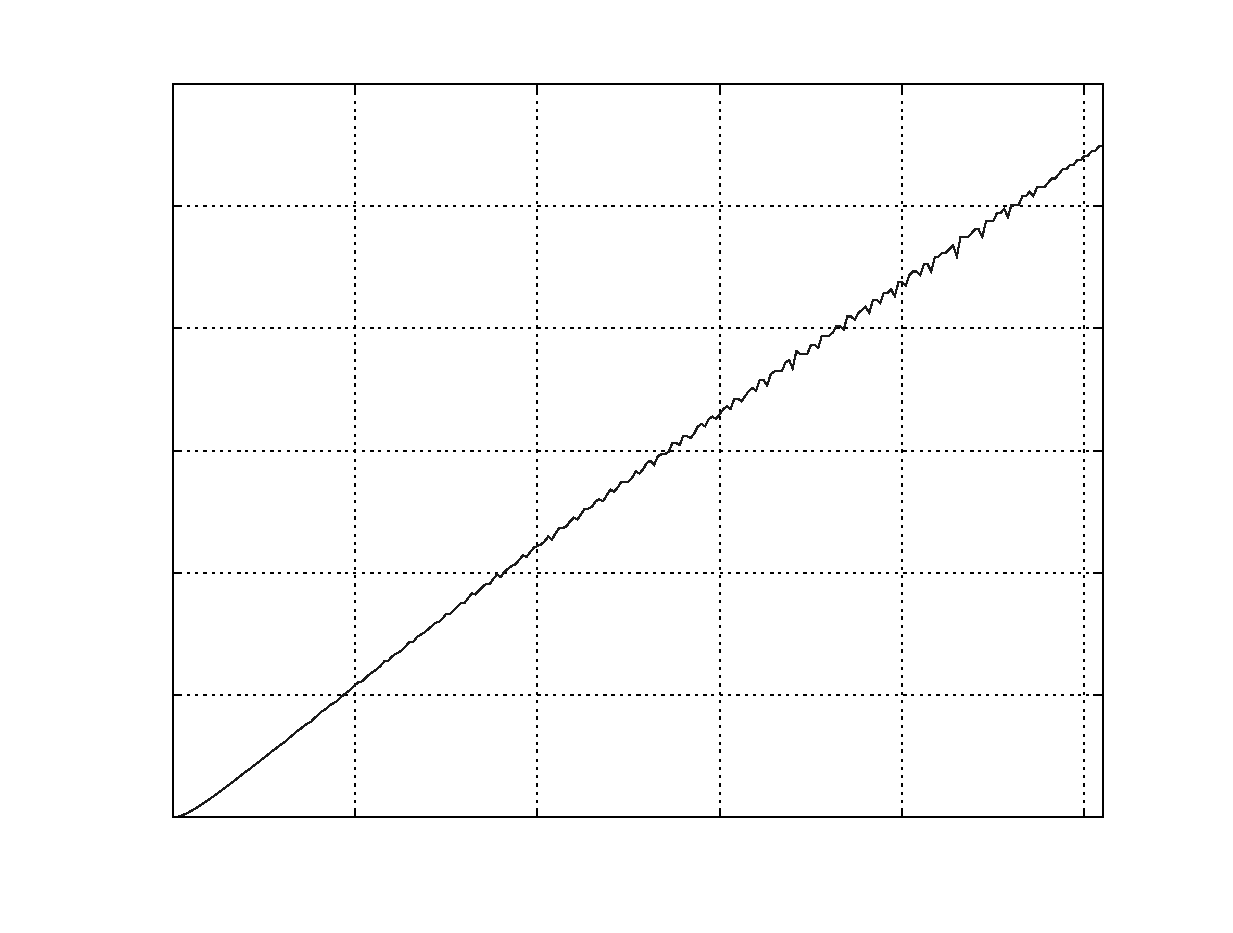
\includegraphics{img/pwm_to_lux-inc}
\end{picture}%
\begin{picture}(576,432)(0,0)
\fontsize{10}{0}
\selectfont\put(74.88,42.5189){\makebox(0,0)[t]{\textcolor[rgb]{0,0,0}{{0}}}}
\fontsize{10}{0}
\selectfont\put(162.409,42.5189){\makebox(0,0)[t]{\textcolor[rgb]{0,0,0}{{50}}}}
\fontsize{10}{0}
\selectfont\put(249.939,42.5189){\makebox(0,0)[t]{\textcolor[rgb]{0,0,0}{{100}}}}
\fontsize{10}{0}
\selectfont\put(337.468,42.5189){\makebox(0,0)[t]{\textcolor[rgb]{0,0,0}{{150}}}}
\fontsize{10}{0}
\selectfont\put(424.998,42.5189){\makebox(0,0)[t]{\textcolor[rgb]{0,0,0}{{200}}}}
\fontsize{10}{0}
\selectfont\put(512.527,42.5189){\makebox(0,0)[t]{\textcolor[rgb]{0,0,0}{{250}}}}
\fontsize{10}{0}
\selectfont\put(69.8755,47.52){\makebox(0,0)[r]{\textcolor[rgb]{0,0,0}{{0}}}}
\fontsize{10}{0}
\selectfont\put(69.8755,106.2){\makebox(0,0)[r]{\textcolor[rgb]{0,0,0}{{10}}}}
\fontsize{10}{0}
\selectfont\put(69.8755,164.88){\makebox(0,0)[r]{\textcolor[rgb]{0,0,0}{{20}}}}
\fontsize{10}{0}
\selectfont\put(69.8755,223.56){\makebox(0,0)[r]{\textcolor[rgb]{0,0,0}{{30}}}}
\fontsize{10}{0}
\selectfont\put(69.8755,282.24){\makebox(0,0)[r]{\textcolor[rgb]{0,0,0}{{40}}}}
\fontsize{10}{0}
\selectfont\put(69.8755,340.92){\makebox(0,0)[r]{\textcolor[rgb]{0,0,0}{{50}}}}
\fontsize{10}{0}
\selectfont\put(69.8755,399.6){\makebox(0,0)[r]{\textcolor[rgb]{0,0,0}{{60}}}}
\fontsize{10}{0}
\selectfont\put(298.08,31.5188){\makebox(0,0)[t]{\textcolor[rgb]{0,0,0}{{PWM value (0--255)}}}}
\end{picture}
}
    \caption{Illuminance detected by the LDR in function of the duty cycle of the LED}
    \label{fig:pwm_to_lux}
\end{figure}


\subsubsection{Step Response}
\label{sub:StepResponse}

To plot the step response of the system an Arduino program was written that to produce a step and acquire data to be ploted. In this script the LED is first turned off for \SI{1}{\second} so that the capacitor ``fully'' discharges. Then a step is applied to the system by setting the LED duty cycle to 0.5. A sample is acquired and sent to the computer approximately every \SI{1.35}{\milli\second}. The readings are converted to Volt and the result is \autoref{fig:step_response}.

An inflection point can be perceived early in the step response. From this follows that the system's order must be at least second degree. The detector in \autoref{fig:setup_LDR_circuit} includes a capacitor, which must introduce a pole. Therefore an experiment was made which consisted simply in removing the capacitor and acquiring the step response again. The result is shown in \autoref{fig:step_response_no_capacitor} where it can be seen that the aforementioned inflection does not exist. It is also noticable that introducing the capacitor does filter high frequency noise, as expected. Therefore introducing the capacitor improves the readings but makes the system order increase. Nonethess the capacitor value can be changed allowing to control the pole position and cutoff frequency.

Assuming that the system can be approximated to a first order system of the form $G(s) = K_0/(1+s\tau)$ the system can be modelled by finding the static gain $K_0$ and the time constant $\tau$. $K_0$ is calculated as the ratio of the output and the input under steady state; the time constant is the time the system takes to reach $1-e^{-1} \approx 63 \%$ of its final value. Therefore for \autoref{fig:step_response} the static gain is $3.08/2.5 = 1.232$ and the time constant is approximately $\SI{23}{\milli\second}$.

If the system is linearised by using the transformation presented in \ref{subsubsec:LDR_model} \autoref{fig:step_response_linearised} is obtained. In this case the static gain is $26.4/2.5 = 10.6$ and the time constant is approximately $\SI{47}{\milli\second}$.

\begin{figure}[h]
    \centering
    \begin{subfigure}[t]{0.49\textwidth}
	\centering
	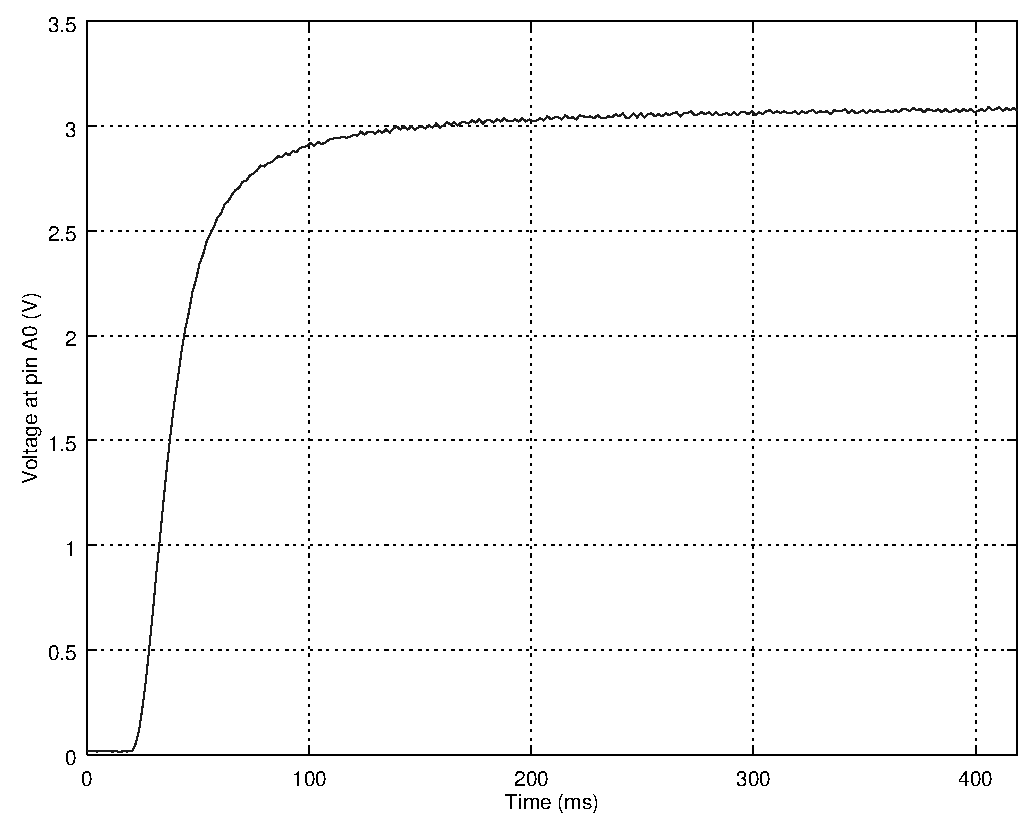
\includegraphics[width=.95\textwidth]{img/step_response}
	\caption{With capacitor, not linearised}
	\label{fig:step_response}
    \end{subfigure}
    \begin{subfigure}[t]{0.49\textwidth}
	\centering
	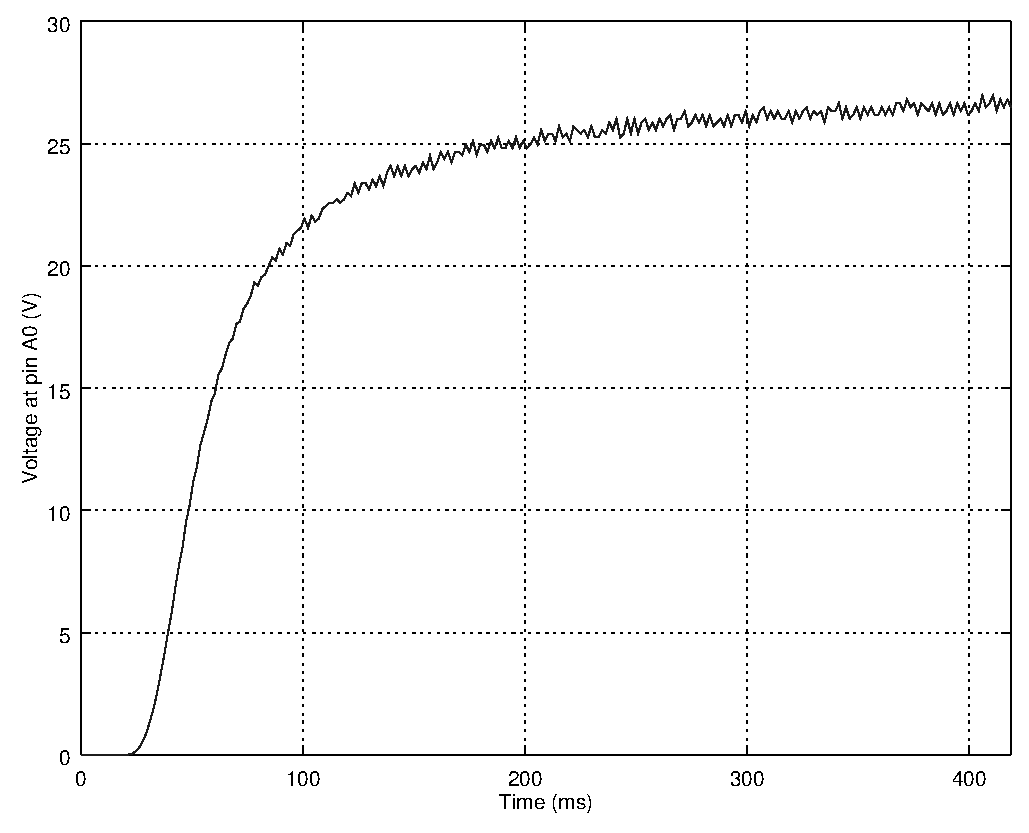
\includegraphics[width=.95\textwidth]{img/step_response_linearised}
	\caption{With capacitor, linearised}
	\label{fig:step_response_linearised}
    \end{subfigure}

    \begin{subfigure}[t]{0.49\textwidth}
	\centering
	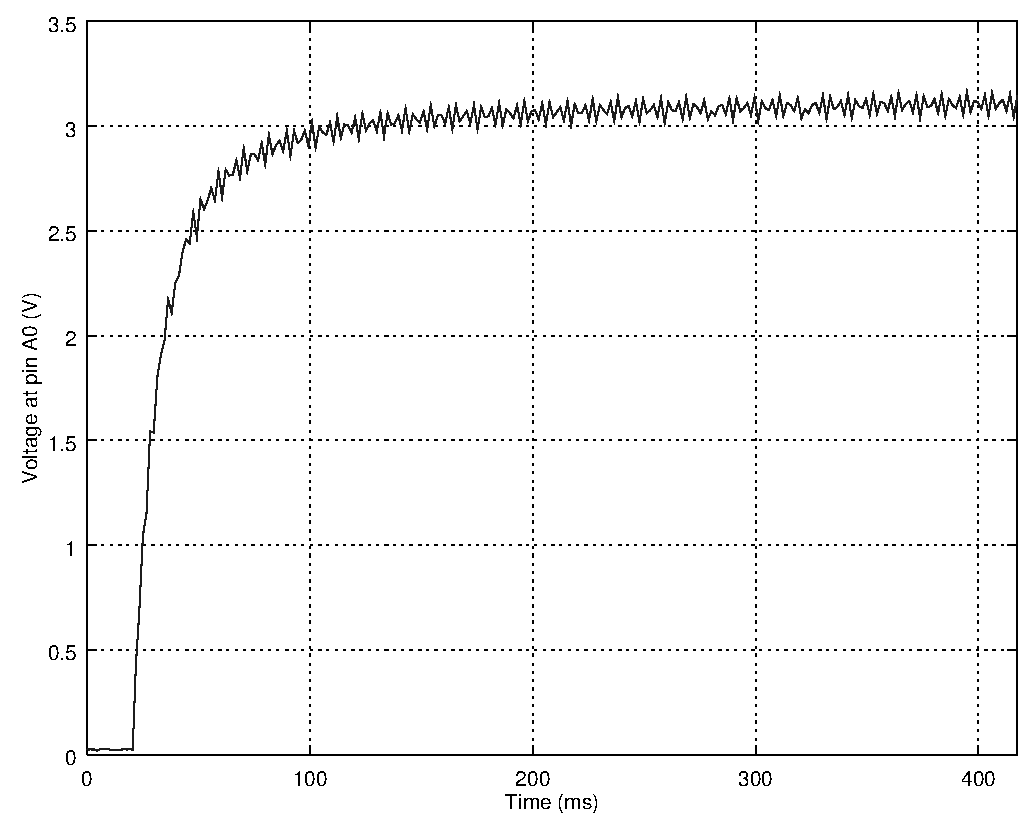
\includegraphics[width=.95\textwidth]{img/step_response_no_capacitor}
	\caption{No capacitor, not linearised}
	\label{fig:step_response_no_capacitor}
    \end{subfigure}
    \caption{Response of the system to a step with 50\% duty cycle applied at time \SI{20}{\milli\second}}
    %\label{fig:}
\end{figure}

\subsubsection{Incremental Response}
\label{sub:IncrementalResponse}

An incremental step response was also produced (\autoref{fig:incstep}). For this, incremental steps of 10 PWM units (3.92\% duty cycle) were used every \SI{400}{\milli\second}. A sample was acquired approximately every \SI{1.35}{\milli\second}.

The acquired data is noisy and therefore it is difficult to measure the time constants for most of the steps. An effort was made to calculate some of the time constants. These results can be seen in \autoref{}. They must be fairly inaccurate.

\begin{figure}[h]
    \begin{subfigure}[t]{0.49\textwidth}
	\centering
	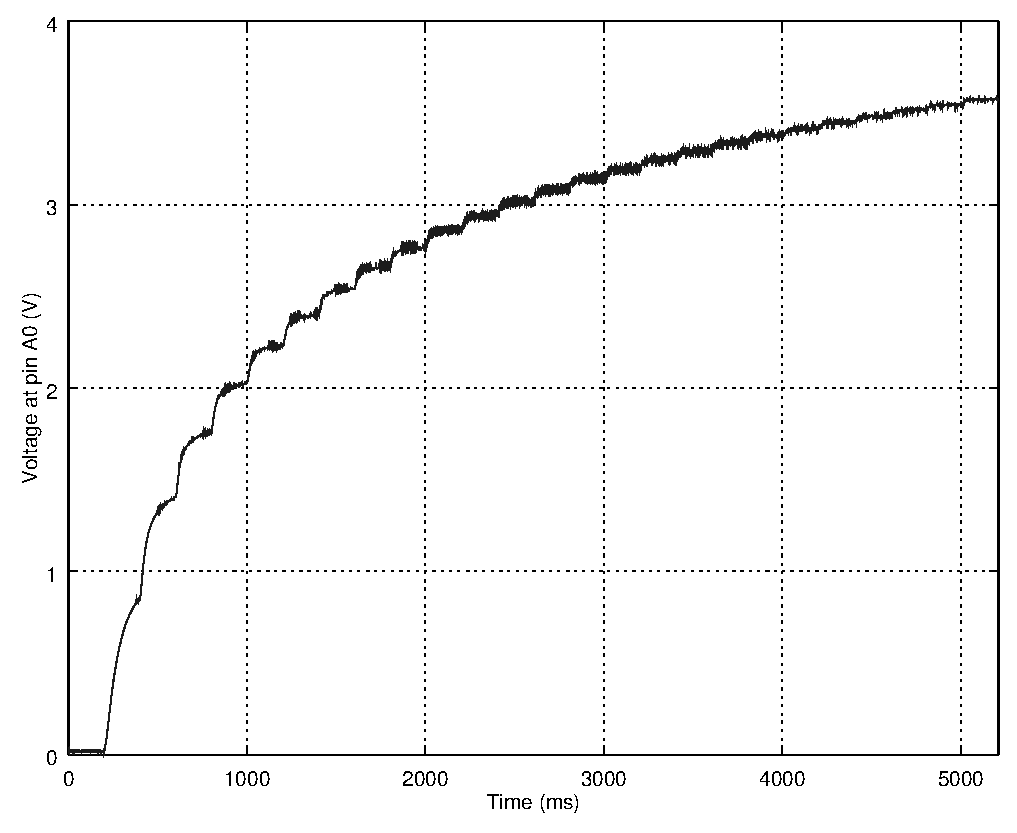
\includegraphics[width=.95\textwidth]{img/incstep_response}
	\caption{Not linearised}
	\label{fig:incstep_response}
    \end{subfigure}
    \begin{subfigure}[t]{0.49\textwidth}
	\centering
	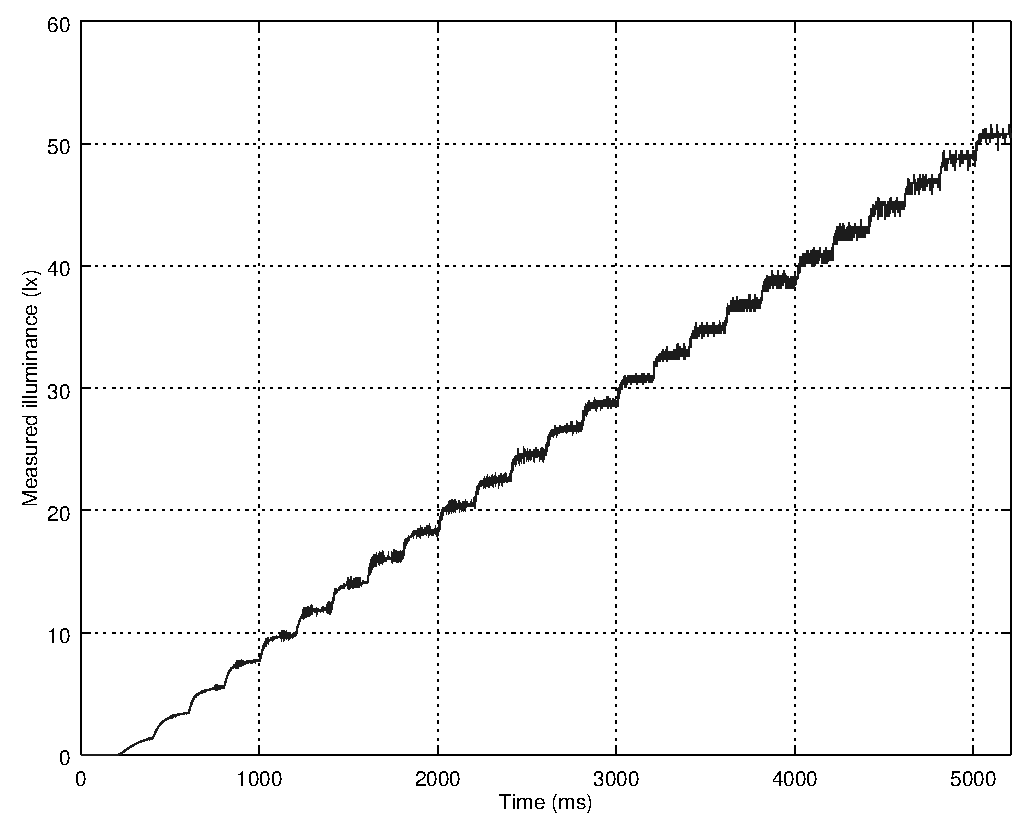
\includegraphics[width=.95\textwidth]{img/incstep_response_linearised}
	\caption{Linearised}
	\label{fig:incstep_response_linearised}
    \end{subfigure}
    \caption{Incremental step responses with increments of 3.92\% duty cycle. First step is at \SI{20}{\milli\second}.}
    \label{fig:incstep}
\end{figure}

% From first report:

%Os seguintes pontos descrevem o que é implementado no código actual:
%Controlador com componentes proporcional, derivativa e integral
%Anti-windup
%Feedforward
%Derivador à saída
%Temporização do controlador através de interrupções
%Dar referências em lux
%Medir iluminância em lux
%Alterar parâmetros do controlador
%Alterar tempo de amostragem
%Implementamos um filtro passa-baixo para o derivador para diminuir o ruído. Não chegámos a afinar a constante desse filtro, pelo que o temos comentado.
%Os parâmetros do controlador foram encontrados com afinação manual e são os seguintes:
%Ganho proporcional: 10
%Ganho diferencial: 0.01
%Ganho integral: 10
%Ganho do feedforward: 0.1
%Ganho do anti-windup: 0.05
%Tempo de amostragem: 1500 µs
%Todos os cálculos do controlador são feitos com valores de 0 a 1023, sendo convertidos quando necessário: para 0 a 255 para actuar o LED; e para lux quando são pedidos valores de iluminância.

\subsection{Local Controller}
\label{sec:LocalController}

The local controller consists of a Proportional-Integral-Derivative Controller (PID) that receives as input a integer reference value (\emph{r}) from 0 to 1023, the LDR readings from 0 to 1023 (\emph{y}) and has as output the PWM duty cycle (\emph{u}) in the range 0 to 255.

The block diagram of the local controller is on Figure~\ref{fig:pid_block_diagramm}. The error(\emph{e}) is defined as $e = r - y$. The signal \emph{u} is calculated as the sum of the proportional, integral and derivative components and the feedforward term.

\subsubsection{Proportional Component}
\label{sub:ProportionalComponent}

The proportional component of the controller is just a gain multiplied (\emph{$K_p$}) by \emph{e}. $ P = K_p * e$.

\subsubsection{Integral Component}
\label{sub:IntegralComponent}

\subsubsection{Derivative Component}
\label{sub:Derivative Component}

The derivative component is calculated as $ D = - K_d/T_s * (y_{t}-y_{t-1})$. This component is calculated with signal \emph{y} instead of \emph{u} to avoid differentiating discontinuities, which would cause the signal \emph{u} to saturate.

\subsubsection{Anti-Windup}
\label{sub:AntiWindup}

\subsubsection{Feedforward}
\label{sub:Feedforward}

\subsubsection{Implementation Details}
\label{sub:Implementation Details}

This controller was implemented as a interrupt routine to guarantee its execution in fixed intervals.

\subsubsection{Parameters}
\label{sub:Parameters}

\section{Server}
\label{sec:Server}

\subsection{Simplex}
\label{sec:Simplex}

The Simplex algorithms solves Linear programms (LP's), it finds a optimal solution if it exists.
We implemented the simplex following the pseudo-code on the book \emph{Introduction to Algorithms} \cite{Cormen}.
This implementation solves Linear programms of the form:

$$ \text{max }c*x $$
$$    A*x \geq b, $$
$$    x \geq 0 $$.

We can describe the problem as a Linear programm of this form. First we define \emph{O} as the array with the external illuminance at each \emph{desk}, \emph{l} as the array with the desired illuminance for each \emph{desk} and \emph{E} as the  3 by 3 matrix of influence between each light.
The problem we want to solve is to find values for \emph{d}, the PWM values normalized from 0 to 1,  minimizing the energy spent and that make the illuminance be equal or greater than \emph{l}.
This can be formalized as:

$$ \text{min }\sum{d} $$
$$    E*d \geq l-O, $$
$$    d \geq 0, $$
$$    d \leq 1 $$.

If we define  $c = [-1, -1, -1]$ we get:

$$ \text{max }c*d $$
$$    E*d \geq l-O, $$
$$    d \geq 0, $$
$$    d \leq 1 $$.

And to remove the last condition we concatenate an identity matrix to the matrix E and an array of 1's to the \emph{l-O} array and get:

??????????????
%TODO: Write the final problem form

I don't know how to write matrices in LaTex and I don't have Internet.

??????????

$$ \text{max }c*d $$
$$    E*d \geq l-O, $$
$$    d \geq 0 $$

With this form we can apply our Simplex algorithm directly.

The Simplex has three possible outcomes.
It may find one of the optimal solutions, the ideal case.
It may detect that there is no possible solution that satisfies all constrains, this happens in our case when we have the illuminance lower than \emph{l} at at least one desk even if all ligths are set to their maximum value.
Or it may declare the problem to be unbounded, where the objective function can have an infinite value, this won't happen in our problem as the maximum value for the objective function would be 0, when all lights are turned off.

Our Simplex implementation has three main routines similarly to the pseudo-code in \cite{Cormen}. The main \emph{Simplex} routine, the \emph{Initialize-Simplex} routine and the \emph{Pivot} routine.

The main routine calls the \emph{Initialize-Simplex} to generate a feasible solution and evaluates it, then makes successive calls to the \emph{Pivot} until it reaches an optimal solution.

The \emph{Initialize-Simplex} routine tests if the initial basic solution (setting \emph{x} to all zero's) is feasible, if not it creates an auxiliary Linear Programm that if it has a solution there is a solution to the initial LP, it then solves the auxiliar LP.

The \emph{Pivot} operation transforms the problem generating a new the solution.

The \emph{Initialize-Simplex} is responsible for detecting if the problem is impossible while the main \emph{Simplex} routine is responsible for detecting if it is unbounded.

Our implementation was able to solve all LP we tested it with, even impossible and unbounded LP's. The results were compared to the \emph{MATLAB: Linear Programming Toolbox}.

\subsubsection{Simplex Implementation Details}
\label{subs:SimplexImplementationDetails}

The Standard C++ library was used widely in the implementation. %TODO: Cite the C++ Standard Library.

Due to possible numerical problems all comparisons within the Simplex implementation are done within a defined \emph{delta}.

To throughly test the Simplex implementation a series of simple unit tests were constructed using the \emph{Boost Test} Library \cite{BoostSite}.

\subsection{Serial Communications}
\label{sec:SerialCommunications}

